    %\setcounter{partie}{0} % Pour s'assurer que le compteur de \partie est à zéro dans les corrigés
    % \phantom{rrr}
    Pour chacune des figure suivantes :

    \begin{itemize}
        \item Préciser le rapport de l'homothétie de centre $O$ qui transforme $M$ en $M_1$.
        \item Préciser, pour chaque homothétie, s'il s'agit d'un agrandissement ou d'une réduction.
    \end{itemize}

    \begin{enumerate}
        \item {\color{red} Rapport : $\dfrac{OM_1}{OM}=2$. Agrandissement.}

        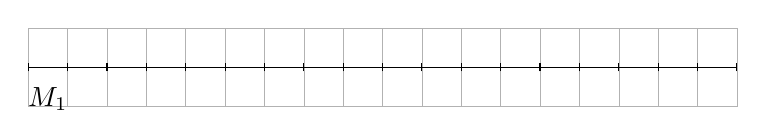
\begin{tikzpicture}[scale=0.5]
            \draw[help lines, color=black!30] (0,0) grid (18,2);
            % Axe
            \draw (0,1)--(18,1);
            \foreach \x in {0,...,18} \draw (\x,0.9) -- (\x,1.1);
            % Points
            \coordinate (O) at (2,1);
            \coordinate (M) at (7,1);
            \tkzDefPointBy[homothety=center O ratio 2](M); \tkzGetPoint{M1};
            % Marques
            \tkzDrawPoints[shape=cross out, size=5pt](O,M,M1);
            \tkzLabelPoints[above](O,M);
            \tkzLabelPoint[above](M1){$M_1$};
        \end{tikzpicture}
        \item {\color{red} Rapport : $\dfrac{OM_1}{OM}=\dfrac{1}{2}$. Réduction.}

        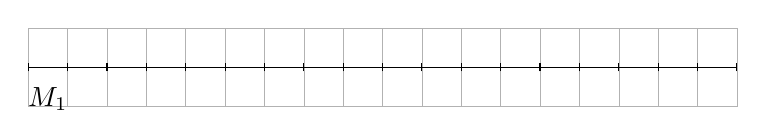
\begin{tikzpicture}[scale=0.5]
            \draw[help lines, color=black!30] (0,0) grid (18,2);
            % Axe
            \draw (0,1)--(18,1);
            \foreach \x in {0,...,18} \draw (\x,0.9) -- (\x,1.1);
            % Points
            \coordinate (O) at (2,1);
            \coordinate (M) at (12,1);
            \tkzDefPointBy[homothety=center O ratio 0.5](M); \tkzGetPoint{M1};
            % Marques
            \tkzDrawPoints[shape=cross out, size=5pt](O,M,M1);
            \tkzLabelPoints[above](O,M);
            \tkzLabelPoint[above](M1){$M_1$};
        \end{tikzpicture}
        \item {\color{red} Rapport : $\dfrac{OM_1}{OM}=\num{1.5}$. Agrandissement.}

        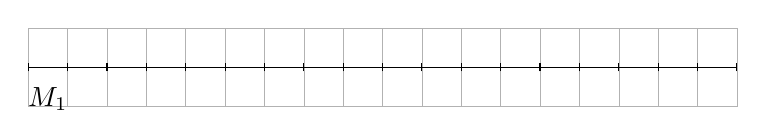
\begin{tikzpicture}[scale=0.5]
            \draw[help lines, color=black!30] (0,0) grid (18,2);
            % Axe
            \draw (0,1)--(18,1);
            \foreach \x in {0,...,18} \draw (\x,0.9) -- (\x,1.1);
            % Points
            \coordinate (O) at (2,1);
            \coordinate (M) at (10,1);
            \tkzDefPointBy[homothety=center O ratio 1.5](M); \tkzGetPoint{M1};
            % Marques
            \tkzDrawPoints[shape=cross out, size=5pt](O,M,M1);
            \tkzLabelPoints[above](O,M);
            \tkzLabelPoint[above](M1){$M_1$};
        \end{tikzpicture}
        \item {\color{red} Rapport : $\dfrac{OM_1}{OM}=\dfrac{3}{4}$. Réduction.}

        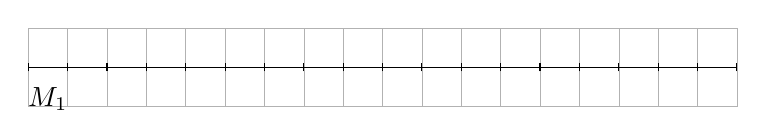
\begin{tikzpicture}[scale=0.5]
            \draw[help lines, color=black!30] (0,0) grid (18,2);
            % Axe
            \draw (0,1)--(18,1);
            \foreach \x in {0,...,18} \draw (\x,0.9) -- (\x,1.1);
            % Points
            \coordinate (O) at (2,1);
            \coordinate (M) at (10,1);
            \tkzDefPointBy[homothety=center O ratio 0.75](M); \tkzGetPoint{M1};
            % Marques
            \tkzDrawPoints[shape=cross out, size=5pt](O,M,M1);
            \tkzLabelPoints[above](O,M);
            \tkzLabelPoint[above](M1){$M_1$};
        \end{tikzpicture}
        \item {\color{red}\small Rapport : $\dfrac{OM_1}{OM}=-1$.  Ni agrandissement, ni réduction.}

        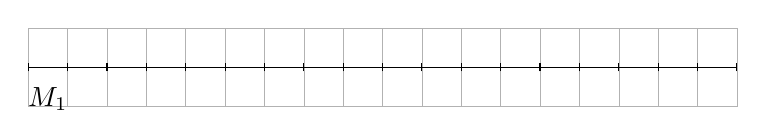
\begin{tikzpicture}[scale=0.5]
            \draw[help lines, color=black!30] (0,0) grid (18,2);
            % Axe
            \draw (0,1)--(18,1);
            \foreach \x in {0,...,18} \draw (\x,0.9) -- (\x,1.1);
            % Points
            \coordinate (O) at (9,1);
            \coordinate (M) at (13,1);
            \tkzDefPointBy[homothety=center O ratio -1](M); \tkzGetPoint{M1};
            % Marques
            \tkzDrawPoints[shape=cross out, size=5pt](O,M,M1);
            \tkzLabelPoints[above](O,M);
            \tkzLabelPoint[above](M1){$M_1$};
        \end{tikzpicture}
        \item {\color{red} Rapport : $\dfrac{OM_1}{OM}=-\dfrac{7}{4}$. Agrandissement.}

        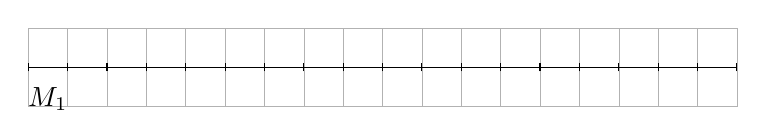
\begin{tikzpicture}[scale=0.5]
            \draw[help lines, color=black!30] (0,0) grid (18,2);
            % Axe
            \draw (0,1)--(18,1);
            \foreach \x in {0,...,18} \draw (\x,0.9) -- (\x,1.1);
            % Points
            \coordinate (O) at (9,1);
            \coordinate (M) at (13,1);
            \tkzDefPointBy[homothety=center O ratio -1.75](M); \tkzGetPoint{M1};
            % Marques
            \tkzDrawPoints[shape=cross out, size=5pt](O,M,M1);
            \tkzLabelPoints[above](O,M);
            \tkzLabelPoint[above](M1){$M_1$};
        \end{tikzpicture}
    \end{enumerate}
